\chapter{Machine learning theory}\label{chap:ml-theory}
\begin{chapterabstract}
This chapter aims to familiarise the reader with the machine learning concepts used within this thesis.
\end{chapterabstract}

\section{Sequence tagging models}
Sequence tagging is an important natural language processing task consisting of receiving a text sequence on input and outputting it tagged. The most famous sequence tagging tasks with defined benchmarks represent, e.g.~part of speech (POS) tagging or named entity recognition (NER) tagging, which aims to identify named entities within a text (people, locations, organizations \ldots).~\cite{BiLSTMCRF}

\subsection{Recurrent neural network (RNN)}
The basic model used for sequence tagging is the recurrent neural network. The RNN model has an input layer $x$, a hidden layer $h$ and an output layer $o$. It maintains a \enquote{memory} (hidden layer $h$) containing preliminary information that enables it to predict the output based on previously seen inputs. In the time step $t$, the following equations are computed:

\begin{gather}
    h_t = f(\mathbf{W}_{xh}x_t + \mathbf{W}_{hh}h_{t-1})\\
    o_t = g(\mathbf{W}_{ho}h_t),
\end{gather}

where
\begin{gather}
    f(z) = \frac{1}{1 + e^{-z}}\\
    g(z_m) = \frac{e^{z_m}}{\sum_{k=1}^{m} e^{z_k}}.
\end{gather}

The input to the input layer at time $t$, $x_t$, is a vector. The hidden layer updates its value by entering the current input $x_t$ and the previous value of the hidden layer $h_{t-1}$ into the sigmoid activation function $f$, which returns values between 0 and 1. The recurrent connection between the previous hidden layers and the current hidden layer represents the \enquote{memory} of the model. An output at time $t$, $o_t$, is a probability distribution over all possible tags. The distribution is obtained from the output of the hidden layer $h_t$ using the softmax activation function $g$. $\mathbf{W}$ represent weight matrices computed during training time.~\cite{BiLSTMCRF} For a graphical illustration of the network, see Figure~\ref{img:rnn}.

\begin{figure}[htbp]
    \centering
    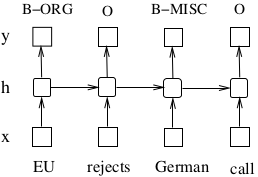
\includegraphics{text/images/rnn.png}
    \caption{RNN~\cite{BiLSTMCRF}}\label{img:rnn}
\end{figure}

\subsection{Long short-term memory network (LSTM)}
Long short-term memory network represents an upgrade of the RNN network that uses a purpose-built memory cell that contains various gates. The memory cell is represented by an input gate $i$, a forget gate $f$, an output gate $o$, and a cell $c$. Due to this approach, LSTM might be more successful than RNN in identifying long-range dependencies in data.

In time $t$ the following equations are computed:
\begin{gather}
    i_t = \sigma(\mathbf{W}_{xi}x_t + \mathbf{W}_{hi}h_{t-1} + \mathbf{W}_{ci}c_{t-1} + b_i)\\
    f_t = \sigma(\mathbf{W}_{xf}x_t + \mathbf{W}_{hf}h_{t-1} + \mathbf{W}_{cf}c_{t-1} + b_f)\\
    c_t = f_tc_{t-1} + i_t\tanh(\mathbf{W}_{xc}x_t + \mathbf{W}_{hc}h_{t-1} + b_c)\\
    o_t = \sigma(\mathbf{W}_{xo}x_t + \mathbf{W}_{ho}h_{t-1} + \mathbf{W}_{co}c_t + b_o)\\
    h_t = o_t\tanh(c_t).
\end{gather}

In the equations, $h$ denotes the hidden vector, $\mathbf{W}$ the weight matrices computed during training, $\sigma$ the sigmoid activation function, and $b$ the bias. The weight matrices from the cell to the gates (e.g.~$\mathbf{W}_{cf}$) are diagonal, and because of this, every element in each gate vector is updated only with the value of the corresponding element in the cell vector.~\cite{BiLSTMCRF}

For an LSTM memory cell schema, see Figure~\ref{img:lstm-cell}. For a network schema, see Figure~\ref{img:lstm}.

\begin{figure}[htbp]
    \centering
    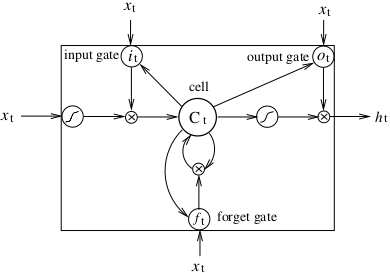
\includegraphics{text/images/lstm_cell.png}
    \caption{LSTM memory cell~\cite{BiLSTMCRF}}\label{img:lstm-cell}
\end{figure}

\begin{figure}[htbp]
    \centering
    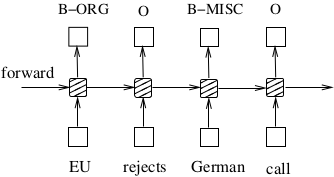
\includegraphics{text/images/lstm.png}
    \caption{LSTM network~\cite{BiLSTMCRF}}\label{img:lstm}
\end{figure}

\subsection{Bidirectional LSTM network (BiLSTM)}
Using RNNs and LSTM networks has one major flaw: for each input, the output is predicted using only the previous input information. Information about future inputs cannot be incorporated. The bidirectional LSTM network solves this problem.

The BiLSTM network contains two LSTM networks: forward, which processes the input sequence from left to right, and backward, which processes it from right to left. The output for a time step is then obtained using information encoded in both networks. The entire network can be trained using the backpropagation through time algorithm.~\cite{BiLSTMCRF} For a network illustration, see Figure~\ref{img:bilstm}.

\begin{figure}[htbp]
    \centering
    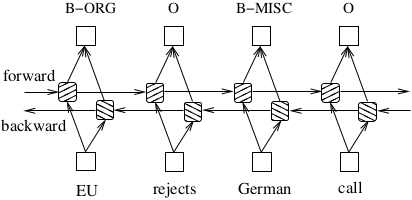
\includegraphics{text/images/bilstm.png}
    \caption{BiLSTM network~\cite{BiLSTMCRF}}\label{img:bilstm}
\end{figure}

\subsection{Conditional random fields network (CRF)}
Unlike the previous approaches, conditional random fields focus on the entire sequence rather than individual positions when finding the optimal tagging. In this model, the inputs and outputs are directly connected. There are no recurrent cells as in the previous approaches (see Figure~\ref{img:crf}).~\cite{BiLSTMCRF} For details, see \cite{CRF}.

\begin{figure}[htbp]
    \centering
    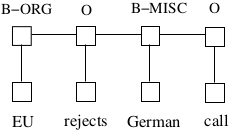
\includegraphics{text/images/crf.png}
    \caption{CRF network~\cite{BiLSTMCRF}}\label{img:crf}
\end{figure}

\subsection{LSTM-CRF network}
LSTM-CRF network combines the LSTM and the CRF network into one model.
When predicting the current tag, it can use information on previous inputs from the LSTM layer, as well as sequence-level information on past and future tags from the CRF layer.~\cite{BiLSTMCRF} For an illustration, see Figure~\ref{img:lstm-crf}.

\begin{figure}[htbp]
    \centering
    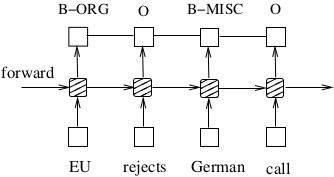
\includegraphics{text/images/lstm_crf.png}
    \caption{LSTM-CRF network~\cite{BiLSTMCRF}}\label{img:lstm-crf}
\end{figure}

\subsection{Bidirectional LSTM-CRF network (Bi\-LSTM-CRF)}
The bidirectional LSTM-CRF network combines the BiLSTM and the CRF network into one model. Unlike the LSTM-CRF network, it uses information about future inputs when predicting the current tag. It represents the current state-of-the-art model for standard sequence tagging tasks such as POS or NER tagging.~\cite{BiLSTMCRF} For an illustration of the network architecture, see Figure~\ref{img:bi-lstm-crf}.

\begin{figure}[htbp]
    \centering
    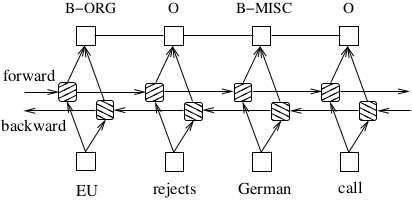
\includegraphics{text/images/bilstm_crf.png}
    \caption{BiLSTM-CRF network~\cite{BiLSTMCRF}}\label{img:bi-lstm-crf}
\end{figure}

\subsubsection{Training procedure}
The BiLSTM-CRF network is trained using the procedure described in Figure~\ref{fig:bi-lstm-crf-trainig}. Multiple training epochs are performed. In each epoch, the training data are divided into equal-sized batches processed independently. First, the BiLSTM network performs forward passes for both its LSTM networks, forward and backward. As a result, the output score $f_{\theta}(w)$ is obtained for all tags at all positions, where $\theta$ represents the parameters of the BiLSTM network and $w$ represents the input sequence. After that, a CRF layer forward and backward passes are run to compute
gradients for the BiLSTM network output and state transition
edges in the CRF layer. The errors are then backpropagated to the input using the backward passes of the BiLSTM network. Finally, all network parameters -- the state transition matrix of the CRF layer and the parameters $\theta$ of the BiLSTM network -- are updated.~\cite{BiLSTMCRF}

\begin{figure}[htbp]
    \centering
  \begin{algorithmic}
    \FOR{each epoch}
        \FOR{each batch}
        \STATE bidirectional LSTM-CRF model forward pass:
            \STATE \quad forward pass for forward state LSTM
            \STATE \quad forward pass for backward state LSTM
        \STATE CRF layer forward and backward pass
        \STATE bidirectional LSTM-CRF model backward pass:
            \STATE \quad backward pass for forward state LSTM
            \STATE \quad backward pass for backward state LSTM
       \STATE update parameters
      \ENDFOR
    \ENDFOR
  \end{algorithmic}
  \caption{BiLSTM-CRF network: Training procedure}\label{fig:bi-lstm-crf-trainig}
\end{figure}

\subsubsection{Input features}
Representation of a word inputted into the BiLSTM-CRF network can consist of multiple concatenated vectors: word embedding, capitalisation feature, and character-based representation.~\cite{BiLSTMCRFHyperparameters} For illustration, see Figure~\ref{img:bi-lstm-crf-input}.

\begin{figure}[htbp]
    \centering
  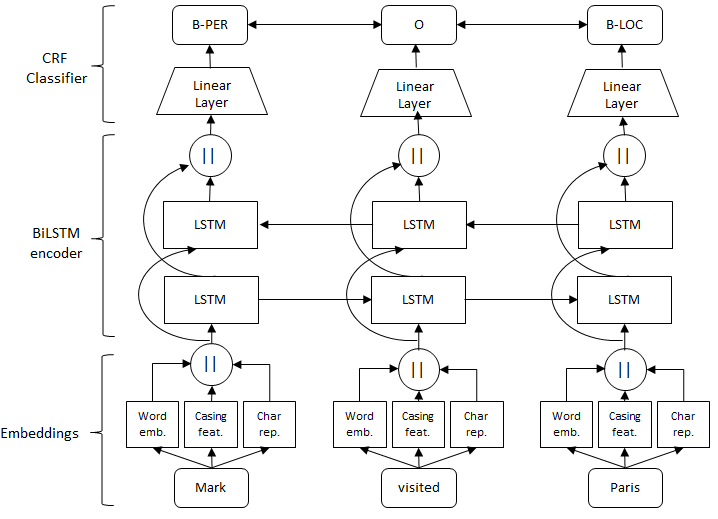
\includegraphics[width=\textwidth]{text/images/bilstm_crf_input.png}
  \caption{BiLSTM-CRF network: Input features~\cite{BiLSTMCRFHyperparameters}}\label{img:bi-lstm-crf-input}
\end{figure}

\paragraph{Word embeddings}
Word embeddings can be used already pre-trained on large text corpora or can be pre-trained on the training data. Popular algorithms for training word embeddings are, for example, GloVe, FastText (which uses n-grams of words)~\cite{BiLSTMCRFHyperparameters}, Word2Vec~\cite{Word2Vec}, or ELMo~\cite{ELMo}.

\paragraph{Capitalisation feature}
Since pre-trained word embeddings usually exist only for lowercase words, a one-hot vector representing the original capitalisation tends to be used. It can preserve information about whether the inputted word is entirely or mainly numeric, has all characters upper or lowercase, starts with an uppercase character, or contains some digit.~\cite{BiLSTMCRFHyperparameters}

\paragraph{Character-based representation}
Information about the characters of a word can also be added to the input. Two different methods can be used: to derive embedding representing characters of a word using BiLSTM or use convolutional neural networks (CNN).~\cite{BiLSTMCRFHyperparameters}

\subsubsection{Training hyperparameters}
When training the BiLSTM-CRF, various hyperparameters of the network can be fine-tuned.

\paragraph{Optimizer}
While training the network, an objective function is minimised using some optimizer. A commonly used optimizer represents stochastic gradient descent (SGD). However, SGD can be quite sensitive to selecting the learning rate and can have trouble navigating ravines and saddle points. Therefore, other gradient-based optimization algorithms have been proposed, such as Adagrad, Adadelta, RMSProp, Adam, or Nadam (Adam variant that incorporates Nesterov momentum).~\cite{BiLSTMCRFHyperparameters}

\paragraph{Dropout}
Dropout is a method that helps prevent overfitting when training a neural network. 

\subparagraph{Naive dropout}
The naive dropout strategy applies a randomly selected dropout mask to each LSTM output. Different masks are generated for each time step, and recurrent connections are not dropped. It was noted that this form of dropout is suboptimal for recurrent neural networks.

\subparagraph{Variational dropout}
The optimal dropout for recurrent neural networks represents the variational dropout. It uses the same dropout mask for all time steps. Moreover, it drops the recurrent connections as well.~\cite{BiLSTMCRFHyperparameters}

\paragraph{Gradient clipping and normalization}
When a recurrent neural network is trained, two common issues can be encountered: \emph{vanishing gradient} and \emph{exploding gradient} problem. The vanishing gradient problem is countered by using LSTM networks instead of RNNs. To deal with the exploding gradient problem, two common strategies can be applied: gradient clipping and gradient normalization.

\subparagraph{Gradient clipping}
Gradient clipping clips the gradient's components element-wise so that they do not exceed a defined threshold.

\subparagraph{Gradient normalization}
Gradient normalization has a better theoretical justification than gradient clipping. It rescales the gradient whenever the norm of the gradient goes over a defined threshold.~\cite{BiLSTMCRFHyperparameters}
